
\chapter{Hardware}
Dieses Kapitel befasst sich mit der im Projekt eingesetzten Hardware.

\section{Allgemeines}
Verwendet wird das STM32F401RE Nucleo Board der Firma STMicroelectronics. Weiterhin wird ein Shield verwendet, welches auf den Microcontroller aufgesteckt werden kann. So wird eine Verbindung zwischen einigen GPIOs des Boards und dem Shield ermöglicht. Des Weiteren werden LEDs und Buttons mitgeliefert. Zuletzt wird noch ein USB-Kabel zur Verbindung zwischen Laptop und Mikrocontroller benötigt. Dieses versorgt den Controller mit Spannung und ermöglicht eine serielle Kommunikation, welche später benötigt wird.

\section{Aufbau}
Im Folgenden wird nun auf den Aufbau der Hardware eingegangen. Das Shield wird auf das Board aufgesteckt. Die mitgelieferten LEDs und Buttons können nun einfach am Shield eingesteckt werden und erhalten damit eine leitende Verbindung zu Versorgungsspannung, Masse und einer Signalleitung. Die Verbindung über das Shield bietet eine höhere Festigkeit und Stabilität gegenüber einzelnen Jumperverbindungen, welche direkt am Board gemacht werden könnten. \\

\begin{figure}[H] 
	\centering
	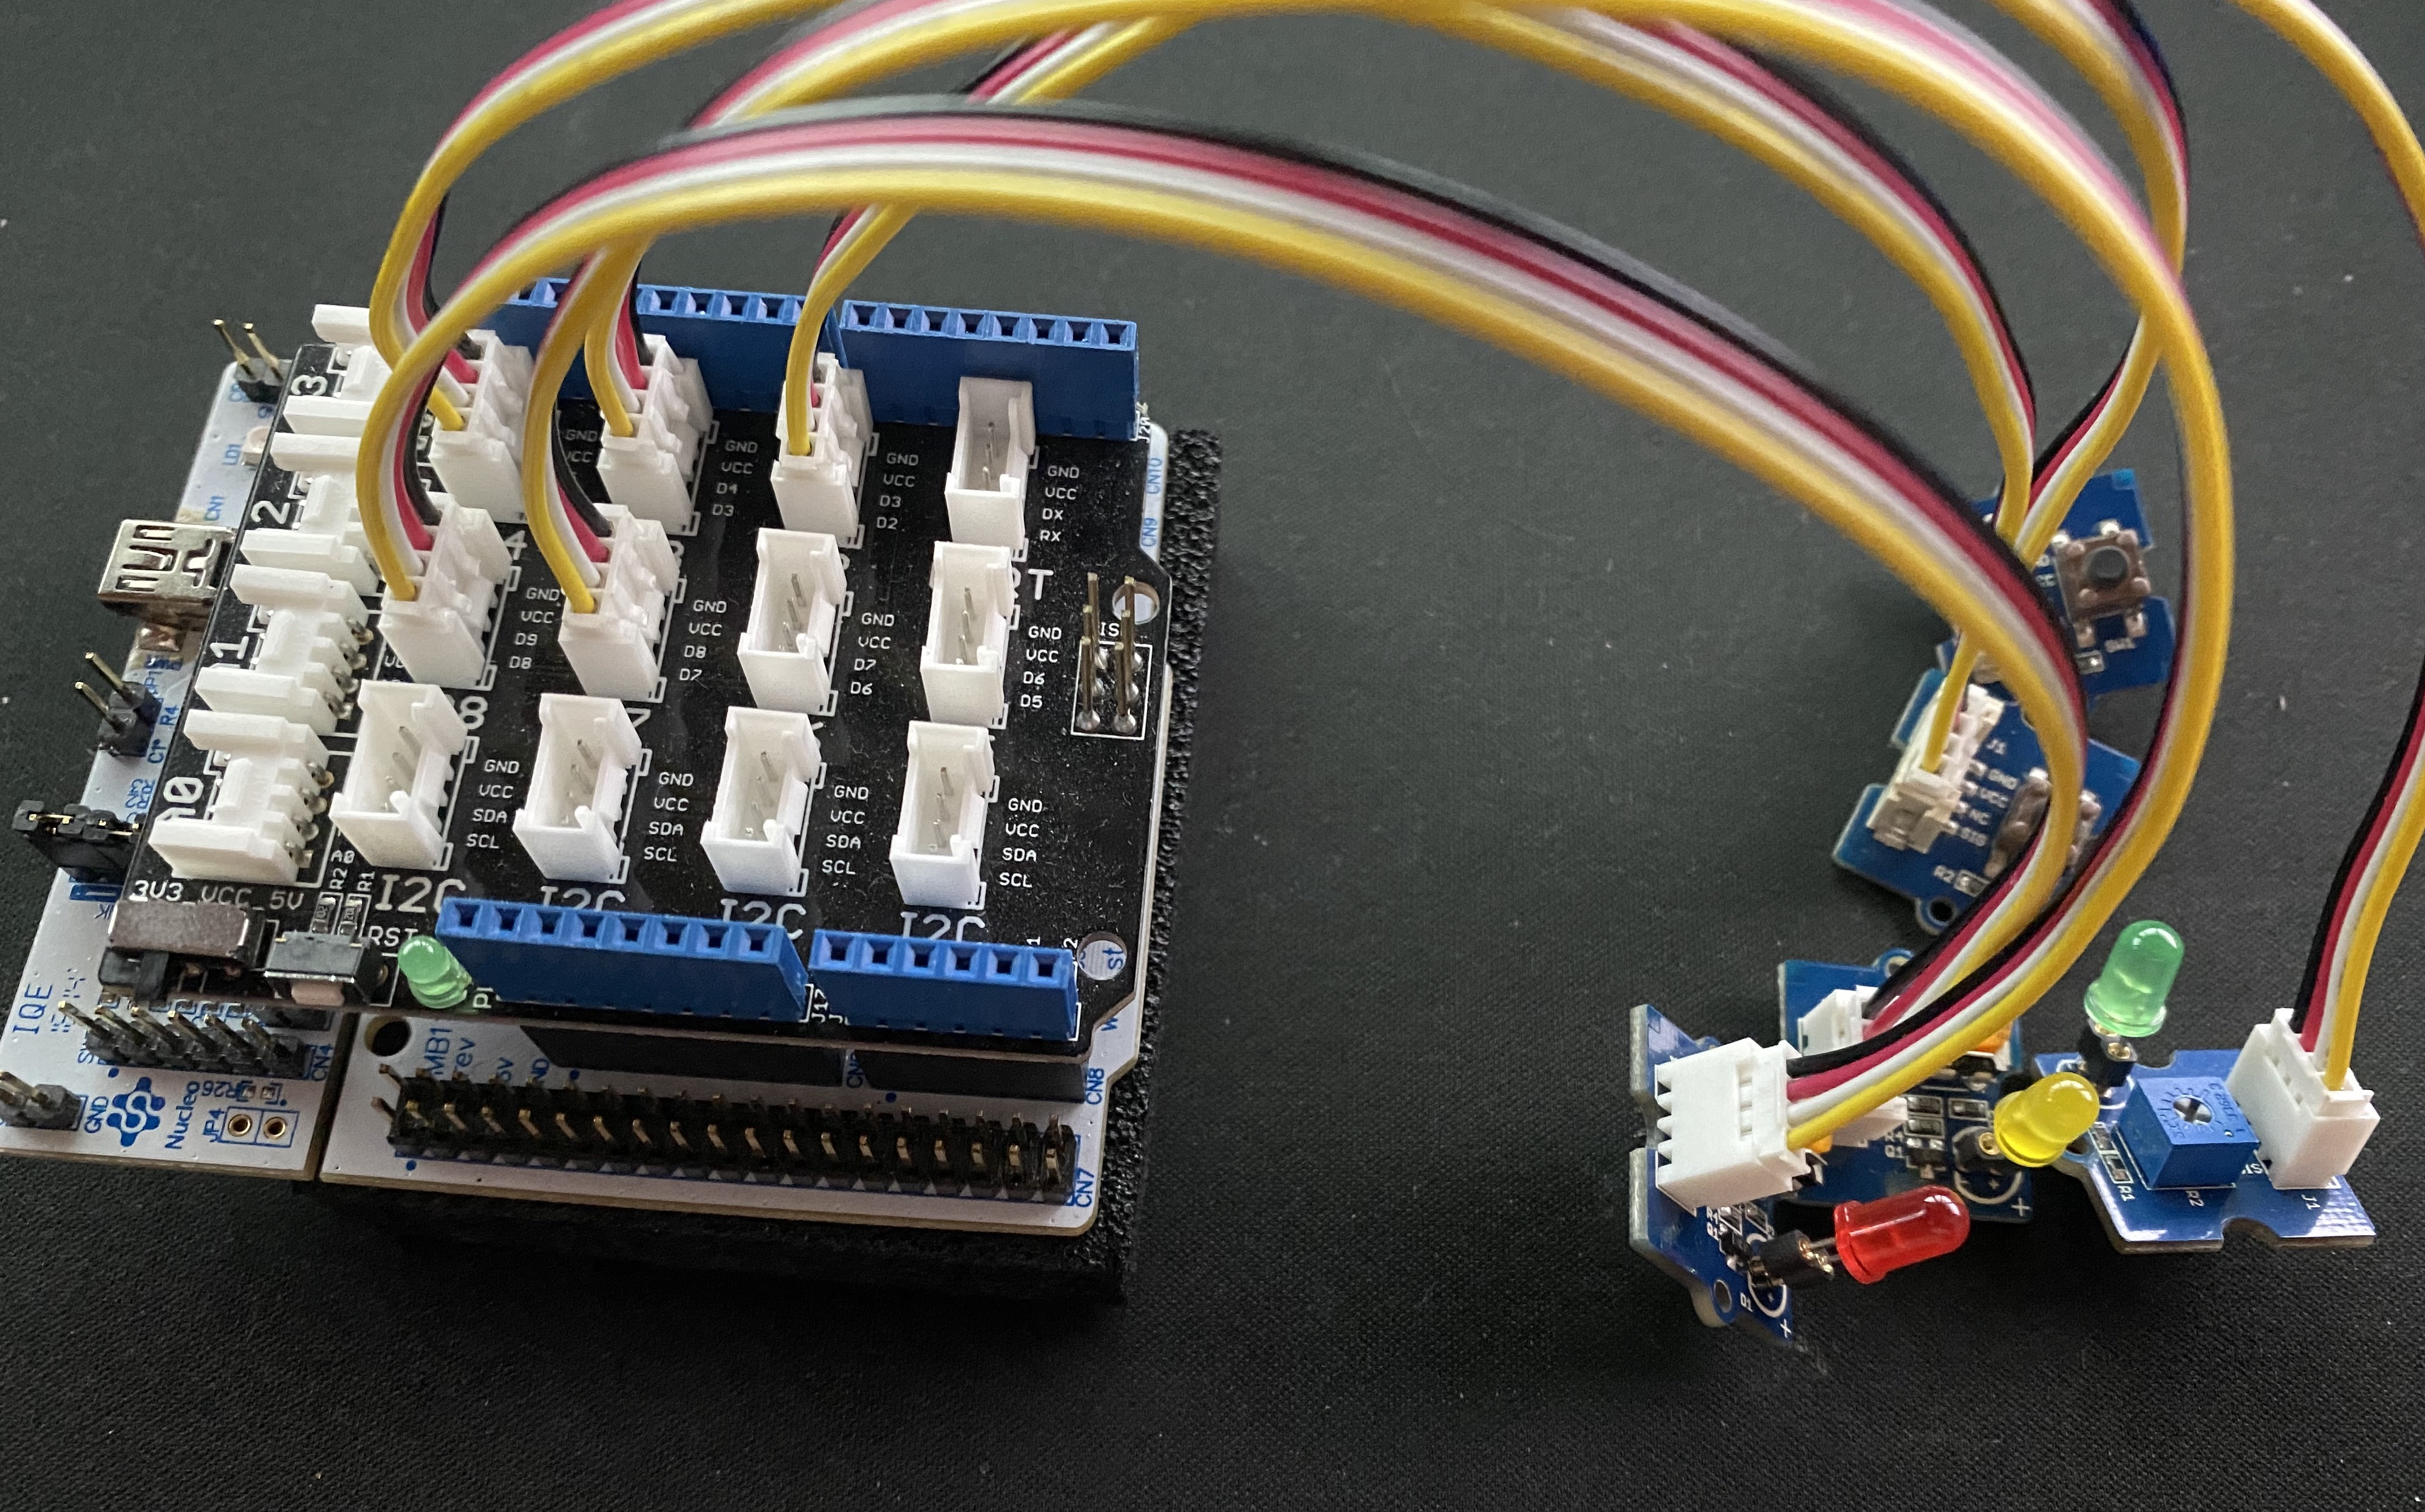
\includegraphics[width=0.38\textwidth]{images/02.png}
	\caption{Hardwareaufbau der Ampelsteuerung  \protect \\ Quelle: Eigene Darstellung }
	\label{fig:grafik2}
\end{figure}


\section{Pinbelegung}
Da der Arbeitsaufwand dieses Projektes auf vier Studierende aufgeteilt wird, muss abgestimmt werden, welcher Pin jeweils den LEDs und den Buttons zugeordnet werden soll. Deshalb wird gleich zu Beginn des Projektes eine Vereinbarung der Pinbelegungen getroffen. Diese ist in \autoref{tab:Pinbelegung} zu sehen.\\

\begin{table}[H]
\centering
\begin{tabular}{c|c|l}
	Hardware - Shield & Software (Port Pin) & Bauteil \\
	\hline
	\rule{0pt}{20pt}D7 & A8 & LED Rot \\
	D8 & A9 & LED Gelb \\
	D2 & A10 & LED Grün \\
	D3 & B3 & Taster 1 \\
	D4 & B5 & Taster 2 \\
	
\end{tabular}
\caption{Pinbelegung (Hardware/Software)}
\label{tab:Pinbelegung}
\end{table}

